\section{Auswertung}
In diesem Kapitel sollen die aufgenommenen Messwerte Ausgewertet und verrechnet werden.
\subsection{Die statische Methode}
\label{sec:auswertung1}
In diesem Kapitel wird die Wärmeleitfähigkeit von verschiedenen Materialien allein durch die Heizkurve bestimmt.

\begin{figure}
    \centering
    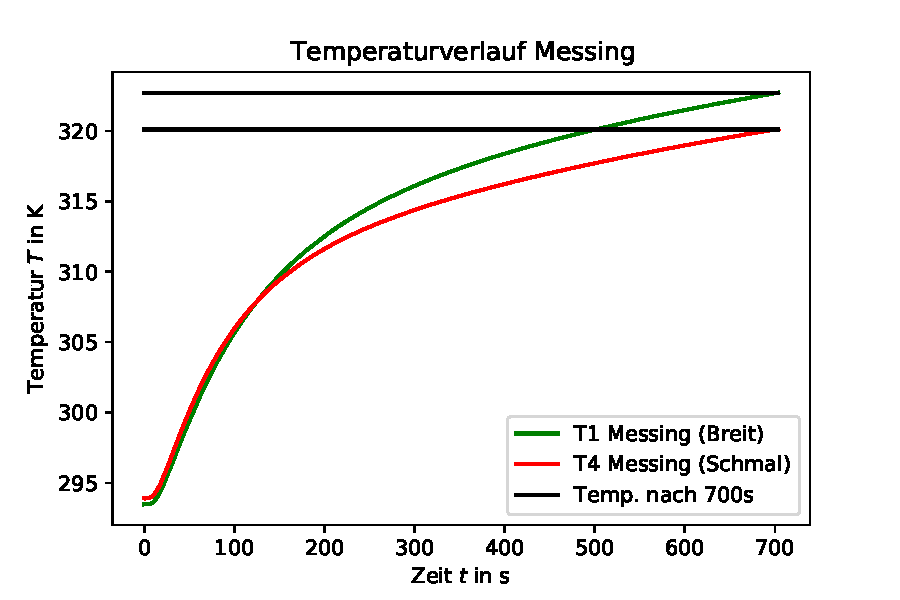
\includegraphics{statmessing.pdf}
    \caption{Zu sehen ist, der statische Temperaturverlauf von Messing.}
    \label{fig:statmess}
  \end{figure}


  \begin{figure}
    \centering
    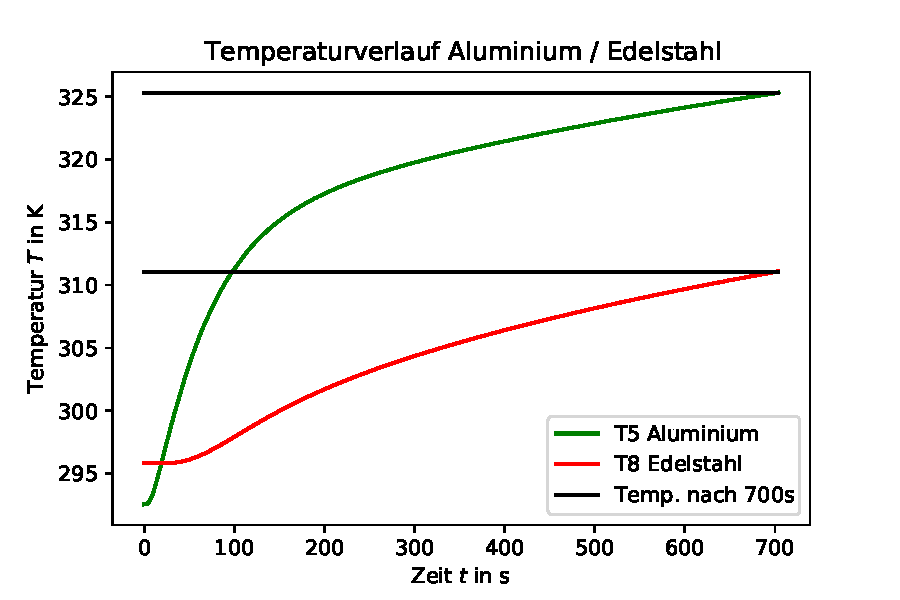
\includegraphics{stataluedel.pdf}
    \caption{Statischer Temperaturverläufe von Aluminium und Edelstahl}
    \label{fig:stataluedel}
  \end{figure}
In \autoref{fig:statmess} und in \autoref{fig:stataluedel} sind die Temperaturverläufe welche an den weiter
vom Heizelement entfernten Temperatursensoren gemessen wurden dargestellt. Zu sehen ist das die Kurven für Messing
am schnellsten ansteigen, die für Aluminium geht bei einer etwas geringeren Temperatur als die Messingkurven 
in ein Plateau über. Der Temperaturverlauf von Edelstahl ist der flachste. Um herauszufinden welcher Metallstab die
beste Wärmeleitung bietet wurden die Temperaturen bei $t=\SI[]{700}[]{s}$ abgelesen, sie sind in
\autoref{tab:siebenhundert} dargestellt. Die höchste Temperatur und damit die beste Wärmeleitfähigkeit hat
demnach Aluminium gefolgt von dem breiten und dem schmalen Messingstab und am Ende dem Edelstahlstab.

  \begin{table}
  \centering
    \caption{Gemessene Temperaturen bei $t=\SI[]{700}[]{s}$.}
    \label{tab:siebenhundert}
    \sisetup{table-format=1.2}
    \begin{tabular}{S[table-format=3.2] S S S S S [table-format=3.2]}
      \toprule
      {Thermoelement Nr} & {Temperatur $T$ in K} &{Material}\\
      \midrule
      1 & {$$322,68$$ }&{Messing (breit)} \\
      4 & {$$320,10$$ }&{Messing (schmal)} \\
      5 & {$$325,28$$ }&{Alluminium} \\
      8 & {$$311,04$$ }&{Edelstahl} \\
      \bottomrule
    \end{tabular}
  \end{table}

  Nun wird für verschiedene Zeiten der Wärmestrom $\frac{\Delta Q}{\Delta t}$ bestimmt.
  \begin{table}
    \centering
      \caption{Hier ist der Wärmestrom in abhängigkeit von der Zeit dargestellt.}
      \label{tab:strom}
      \sisetup{table-format=1.2}
      \begin{tabular}{S[table-format=3.2] S S S S S [table-format=3.2]}
        \toprule
        {Zeitpunkt $t$} &{$(\frac{\Delta Q}{\Delta t})_{Mb} / Wm$} &{$(\frac{\Delta Q}{\Delta t})_{Ms} / Wm$}&{$(\frac{\Delta Q}{\Delta t})_{A} / Wm$}&{$(\frac{\Delta Q}{\Delta t})_{E} / Wm$}\\
        \midrule
        {$$140,8$$} &{$$0,00927$$}&{$$0,01129$$}&{$$0,00639$$}&{$$0,00600$$} \\
        {$$281,6$$} &{$$0,00570$$}&{$$0,00804$$}&{$$0,00405$$}&{$$0,00545$$} \\
        {$$422,4$$} &{$$0,00468$$}&{$$0,00733$$}&{$$0,00359$$}&{$$0,00511$$} \\
        {$$563,2$$} &{$$0,00439$$}&{$$0,00720$$}&{$$0,00345$$}&{$$0,00493$$} \\
        {$$703,8$$} &{$$0,00432$$}&{$$0,00716$$}&{$$0,00341$$}&{$$0,00483$$} \\
        \midrule
        {$$\diameter$$}&{$$0,0057\pm 0,0009$$}&{$$0,0082\pm 0,0008$$}&{$$0,0042\pm 0,0006$$}&{$$0,00527\pm 0,00021$$}\\
        
        \bottomrule
      \end{tabular}
    \end{table}
Die in \autoref{tab:strom} berechneten Mittelwerte und entsprechende Fehler wurden nach \autoref{eq:Mittelwert} 
und \autoref{eq:mittelwertfehler} berechnet.
In \autoref{fig:differenz1} ist die Differenz der beiden Temperatursensoren des Messingstabes
aufgetragen und in \autoref{fig:differenz2} ist die Differenz der Temperatursensorendes Edelstahlstabes  aufgetragen.
Hier fällt auf das der Messingstab die Wärme viel schneller leitet und so die Tepmeraturdifferenz sehr viel schneller
kleiner wird.  
    \begin{figure}
        \centering
        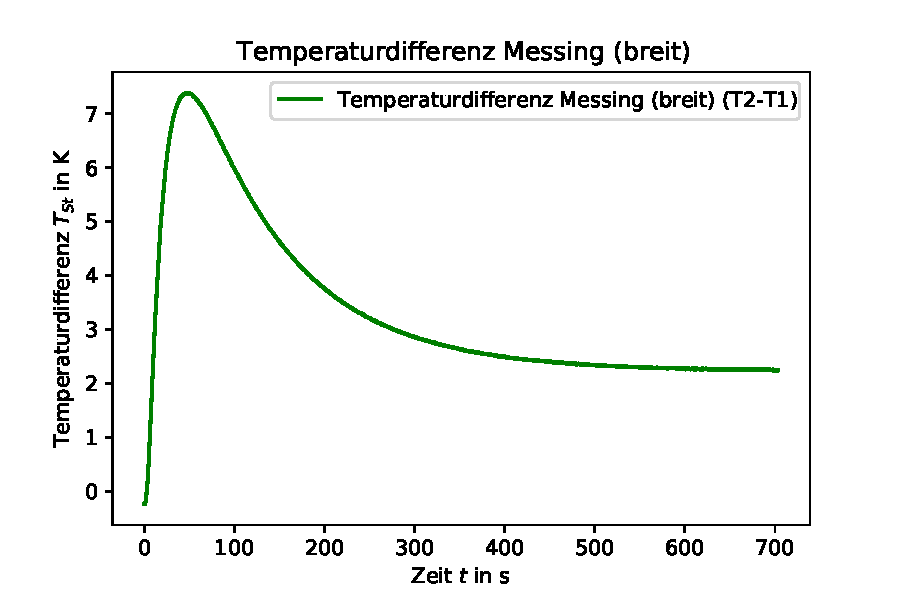
\includegraphics{diffmess.pdf}
        \caption{Temperaturdifferenzverlauf von Messing.}
        \label{fig:differenz1}
      \end{figure}
    \begin{figure}
        \centering
        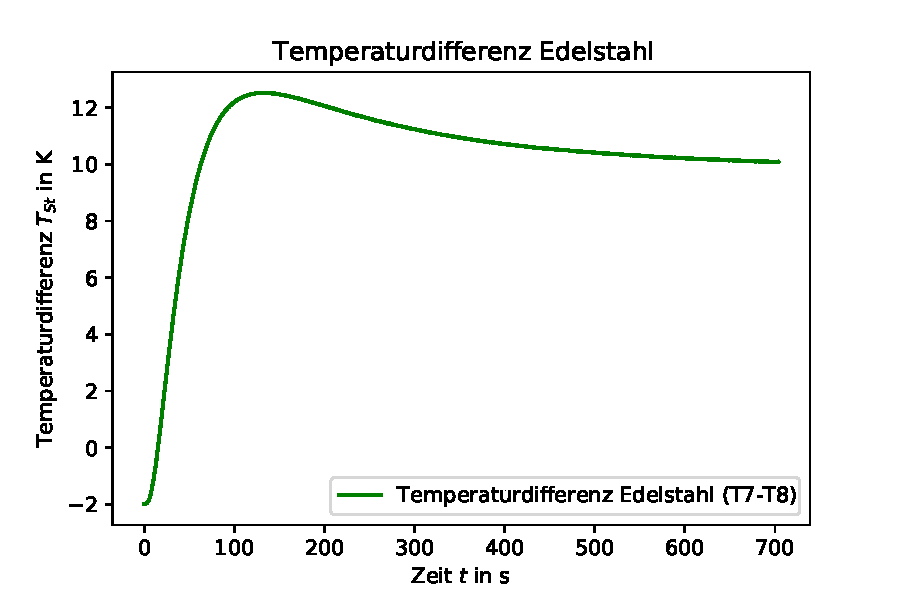
\includegraphics{diffed.pdf}
        \caption{Temperaturdiffernzverlauf von Edelstahl.}
        \label{fig:differenz2}
      \end{figure}

\subsection{Das Angström Messverfahren}
\label{sec:auswertung2}
In diesem Schritt werden die Wärmeleitfähigketen $\kappa$ mit dem Angström Messverfahren 
also durch abwechselndes erhitzen und Kühlen der Stäbe genutzt. Dabei wird eine 
Periodendauer von $T=\SI[]{80}[]{s}$ verwendet. Die Temperaturverläufe sind in 
\autoref{fig:wellmess} für Messing und in \autoref{fig:aluwelle} für Aluminium dargestellt.


\begin{figure}
    \centering
    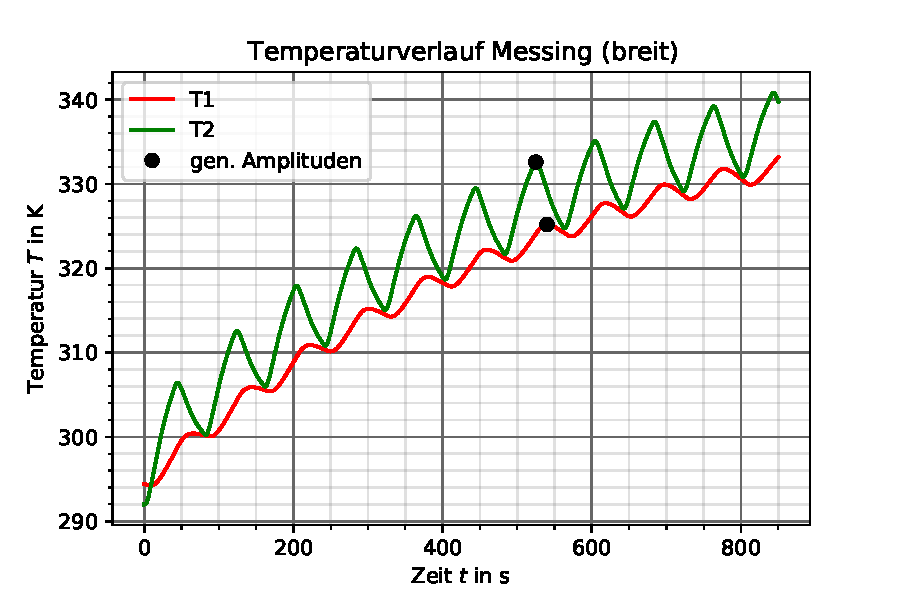
\includegraphics{wellemessing.pdf}
    \caption{In dieser Grafik ist derTemperaturverlauf des breiten Messingstabes im Angström-Verfahren.}
    \label{fig:wellmess}
  \end{figure}

  \begin{figure}
    \centering
    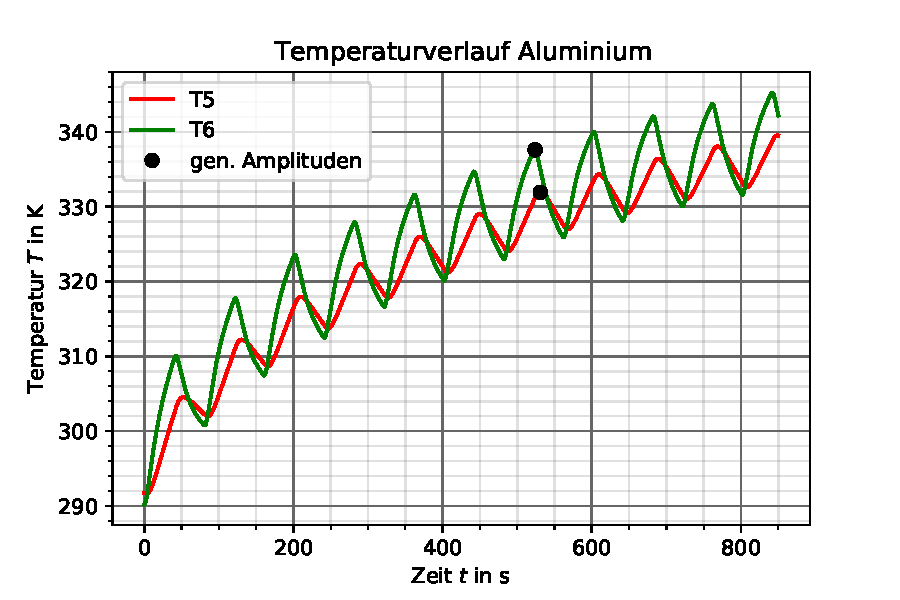
\includegraphics{wellenalu.pdf}
    \caption{Hier ist der Temperaturverlauf von Aluminium im Angström-Verfahren dargestellt.}
    \label{fig:aluwelle}
  \end{figure}

  \begin{figure}
    \centering
    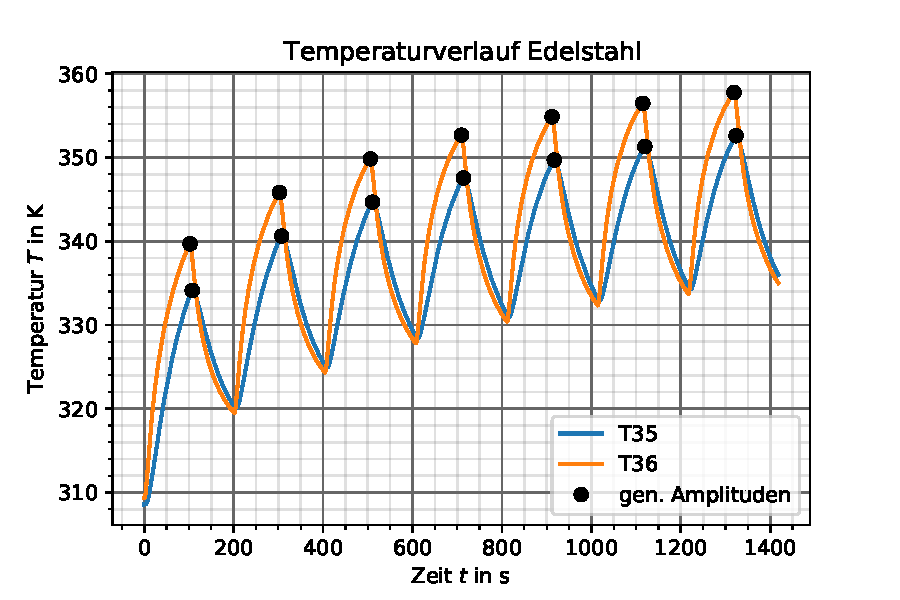
\includegraphics{welleedelstahl.pdf}
    \caption{Temperaturverlauf von Edelstahl im Angström-Verfahren zu sehen.}
    \label{fig:edelwelle}
  \end{figure}



  Mit den gekenzeichneten Amplituden folgen sofort die Phasenverschiebungen und Amplitudenvergältnisse
  welche für Messing in \autoref{tab:wertemessing}, für Aluminium in \autoref{tab:wertealu} und für 
  Edelstahl in \autoref{tab:werteedelstahl} dargestellt. Die ebenfalls in den Tabellen dargestellten
  Werte für $\kappa$ wurden einzeln über \autoref{eq:sechs} berechnet und anschließend über \autoref{eq:Mittelwert} gemittelt
  und der Fehler mit \autoref{eq:mittelwertfehler} berechnet.

  \begin{table}
    \centering
      \caption{Verschiedene Werte zur berechnung von $\kappa$ für Messing.}
      \label{tab:wertemessing}
      \sisetup{table-format=1.2}
      \begin{tabular}{S[table-format=3.2] S S S S S [table-format=3.2]}
        \toprule
        {Nr.}&{ $\Delta t$ / s}&{ $\frac{A_{nah}}{A_{fern}}$ }&{ $\kappa$ / $\si[]{\frac{kW}{K*m}}$}\\
        \midrule
        {1}&{$$21$$}&{$$1,0199$$}&{$$3,5543$$}\\
        {2}&{$$20$$}&{$$1,0218$$}&{$$3,4114$$}\\
        {3}&{$$17$$}&{$$1,0226$$}&{$$3,8719$$}\\
        {4}&{$$18$$}&{$$1,0227$$}&{$$3,6507$$}\\
        {5}&{$$17$$}&{$$1,0227$$}&{$$3,8634$$}\\
        {6}&{$$16$$}&{$$1,0227$$}&{$$4,1123$$}\\
        {7}&{$$14$$}&{$$1,0228$$}&{$$4,6794$$}\\
        {8}&{$$14$$}&{$$1,0226$$}&{$$4,7217$$}\\
        {9}&{$$14$$}&{$$1,0225$$}&{$$4,7282$$}\\
        {10}&{$$14$$}&{$$1,0224$$}&{$$4,7605$$}\\
        \midrule
        {$$\diameter$$}&{$$$$}&{$$$$}&{$$4,14\pm 0,17$$}\\

        \bottomrule
      \end{tabular}
    \end{table}

    \begin{table}
      \centering
        \caption{Verschiedene Werte zur berechnung von $\kappa$ für Aluminium.}
        \label{tab:wertealu}
        \sisetup{table-format=1.2}
        \begin{tabular}{S[table-format=3.2] S S S S S [table-format=3.2]}
          \toprule
          {Nr.}&{ $\Delta t$ / s}&{ $\frac{A_{nah}}{A_{fern}}$ }&{ $\kappa$ / $\si[]{\frac{kW}{K*m}}$}\\
          \midrule
          {1}&{$$11$$}&{$$1,0180$$}&{$$5,3312$$}\\
          {2}& {$$9$$}&{$$1,0177$$}&{$$6,6072$$}\\
          {3}& {$$8$$}&{$$1,0176$$}&{$$7,5013$$}\\
          {4}& {$$8$$}&{$$1,0174$$}&{$$7,5896$$}\\
          {5}& {$$8$$}&{$$1,0172$$}&{$$7,6614$$}\\
          {6}& {$$8$$}&{$$1,0172$$}&{$$7,6648$$}\\
          {7}& {$$7$$}&{$$1,0171$$}&{$$8,8049$$}\\
          {8}& {$$7$$}&{$$1,0169$$}&{$$8,9147$$}\\
          {9}& {$$7$$}&{$$1,0169$$}&{$$8,9386$$}\\
          {10}&{$$7$$}&{$$1,0168$$}&{$$8,9821$$}\\
          \midrule
          {$$\diameter$$}&{$$$$}&{$$$$}&{$$7,8\pm 0,4$$}\\
          \bottomrule
        \end{tabular}
      \end{table}
  
      
      \begin{table}
        \centering
          \caption{Verschiedene Werte zur berechnung von $\kappa$ für Edelstahl.}
          \label{tab:werteedelstahl}
          \sisetup{table-format=1.2}
          \begin{tabular}{S[table-format=3.2] S S S S S [table-format=3.2]}
            \toprule
            {Nr.}&{ $\Delta t$ / s}&{ $\frac{A_{nah}}{A_{fern}}$ }&{ $\kappa$ / $\si[]{\frac{kW}{K*m}}$}\\
            \midrule
            {1}&{$$5,5$$}&{$$1,0166$$}&{$$15,8641$$}\\
            {2}&{$$5,5$$}&{$$1,0153$$}&{$$17,2478$$}\\
            {3}&{$$5,0$$}&{$$1,0150$$}&{$$19,3438$$}\\
            {4}&{$$5,5$$}&{$$1,0147$$}&{$$17,9030$$}\\
            {5}&{$$5,0$$}&{$$1,0148$$}&{$$19,6235$$}\\
            {6}&{$$5,0$$}&{$$1,0147$$}&{$$19,7132$$}\\
            {7}&{$$4,5$$}&{$$1,0146$$}&{$$22,0687$$}\\

            \midrule
          {$$\diameter$$}&{$$$$}&{$$$$}&{$$18,8\pm 0,8$$}\\
          \bottomrule
        \end{tabular}
      \end{table}
  
      
  Dazu wurde $\Delta x=\SI[]{0,03}[]{m}$ verwendet.
  

  

  Die Wellenlängen und Frequenzen lassen sich einfach bestimmen mit den Zusammenhängen:
  \begin{center}
      $\omega=\frac{2\pi}{T}$,\\
      $v=\sqrt{\frac{2\kappa \omega}{\rho c}}$,\\
      $\lambda=\frac{2\pi v}{\omega}.$
\end{center}
Die gemessenen und über \autoref{eq:Mittelwert} gemittelten Periodendauern $T$ sind in \autoref{tab:periodendauern}
dargestellt. Der Fehler des Mittelwertes berechnet sich wieder über \autoref{eq:mittelwertfehler}.
\begin{table}
  \centering
    \caption{Periodendauern der Metalle Messing, Alluminium und Edelstahl.}
    \label{tab:periodendauern}
    \sisetup{table-format=1.2}
    \begin{tabular}{S[table-format=3.2] S S S S S [table-format=3.2]}
      \toprule
      {Nr.}&{ $T_{Messing}$ / s}&{ $T_{Aluminium}$ / s }&{$T_{Edelstahl}$ / s }\\
      \midrule
      {1}&{$$78$$}&{$$78$$}&{$$200,0$$}\\
      {2}&{$$77$$}&{$$79$$}&{$$203,0$$}\\
      {3}&{$$81$$}&{$$80$$}&{$$204,0$$}\\
      {4}&{$$79$$}&{$$80$$}&{$$202,5$$}\\
      {5}&{$$79$$}&{$$80$$}&{$$202,5$$}\\
      {6}&{$$80$$}&{$$81$$}&{$$204,0$$}\\
      {7}&{$$79$$}&{$$79$$}&{$$$$}\\
      {8}&{$$79$$}&{$$79$$}&{$$$$}\\
      {9}&{$$80$$}&{$$80$$}&{$$$$}\\
      \midrule
      {$$\diameter$$}&{$$79,1\pm 0,4$$}&{$$79,56\pm 0,29$$}&{$$202,7\pm 0,6$$}\\
      \bottomrule
    \end{tabular}
  \end{table}


  




Daraus folgen sofort die Ergebnisse in \autoref{tab:ergebnisse} deren Fehler sich über \autoref{eq:gaussfehler} ergibt.
\begin{table}
    \centering
      \caption{Die Ergebnisse der Rechnungen.}
      \label{tab:ergebnisse}
      \sisetup{table-format=1.2}
      \begin{tabular}{S[table-format=3.2] S S S S S [table-format=3.2]}
        \toprule
        {Material}&{ $T$ / s}&{ $\omega$ / 1/s}&{ $v$ / m/s}&{ $f$ / Hz}&{ $\lambda$ / m}\\
        \midrule
        {Messing (breit)}&{$$79,1\pm 0,4$$}  &{$$0,0794\pm 0,0004$$}  &{$$0,0142\pm 0,0003$$} &{$$0.01264\pm 0.00006$$}&{$$1,12\pm 0,023$$} \\
        {Alluminium}     &{$$79,56\pm 0,29$$}&{$$0,0789\pm 0,0003$$}  &{$$0,0230\pm 0,0006$$} &{$$0.01257\pm 0.00005$$}&{$$1,83\pm 0,04$$}  \\
        {Edelstahl}      &{$$202,7\pm 0,6$$} &{$$0,0310\pm 0,00009$$} &{$$0,0191\pm 0,0004$$} &{$$0.00493\pm 0.00002$$}&{$$3,87\pm 0,08$$}  \\
        \bottomrule
      \end{tabular}
    \end{table}

    